\documentclass{report}
\usepackage{ptext}
\usepackage{lipsum}
\usepackage{graphicx}
\usepackage{ptext}

\input{Boostan-UserManual}

\newword{Abstraction}{Abstraction}
{انتزاع}{}

\newword{Abstract}{Abstract}
{انتزاعی}{}

\newword{AbsoluteMinimum}{Absolute Minimum}
{کمینه مطلق}{}


\newword{AcceptableCell}{Acceptable Cell}
{سلول پذیرفتنی}{سلول‌های پذیرفتنی}

\newword{AccessBurst}{Access Burst}
{توده دسترسی}{توده‌های دسترسی}


%%% S
\newword{Sample}{Sample}
{نمونه}{نمونه‌ها}

\newword{SamplePath}{Sample Path}
{نمونه مسیر}{}

\newword{SampleSpace}{Sample Space}
{فضای نمونه}{فضای نمونه‌ها}
\newacronym{ACK}{ACK}{Acknowledgement}

\newacronym{ACI}{ACI}{Application Control Interface}

\newacronym{ACIR}{ACIR}{Adjacent Channel Interference Ratio}

\newacronym{ACLC}{ACLC}{Adaptive Configuration of Logical Channels}

\newacronym{ACLP}{ACLP}{Adjacent Channel Leakage Power}

\title{مستند راه اندازی پروژه نهایی درس شبکه های تلفن همراه}
\type{مستند }
\author{زهرا دهقان\\اسماء حمید\\فاطمه شرح دهی مقدم}

\logofile{Pic/logo}


\begin{document}

\pagenumbering{gobble}
\Godpage
\maketitle
\pagenumbering{arabic}
\tableofcontents


\chapter{مقدمه}








\chapter{ \lr{Server-side Component}}

\chapter{ \lr{Web Application}}

\chapter{ \lr{Android Mobile}}

\section{پیکربندی و راه‌اندازی اولیه اپلیکیشن}

برای اتصال اپلیکیشن به بک‌اند در محیط محلی، بک‌اند و موبایل باید در یک شبکه باشند. سپس آدرس IP سیستم میزبان بک‌اند را با دستور \textbf{ipconfig} در CMD پیدا کنید. آدرس \lr{IPv4} را یادداشت کرده و در محل زیر جایگزین کنید:

	مسیر: \\
	\begin{latin}
		\texttt{app/src/main/java/com/example/Havanet/viewmodels/SharedViewModel.kt}\\
	\end{latin}
	مقدار موجود در خط شماره پانزده، عبارت از:
\begin{latin}
\begin{lstlisting}[mathescape=true, numbers=left, firstnumber=15]
val ip = "10.13.148.180"
\end{lstlisting}
\end{latin}
	را با IP جدید جایگزین کنید.لطفاً دقت داشته باشید که پورت 8000 روی دستگاه شما باز باشد.

	

\vspace{0.5cm}

پس از انجام مراحل فوق، اپلیکیشن را با استفاده از \lr{Android Studio} روی دستگاه نصب کنید.

\section{مجوزهای موردنیاز}

اپلیکیشن برای عملکرد صحیح به مجوزهای مختلف نیاز دارد. برخی از این مجوزها هنگام اجرا از کاربر درخواست تأیید می‌شوند و باید آنها را قبول کند تا امکانات مربوط فعال شوند.

مجوزهای زیر هنگام اجرای برنامه از کاربر درخواست می‌شوند و باید حتماً اجازه داده شوند:

\begin{itemize}
	\item \lr{ACCESS\_FINE\_LOCATION}
	\item \lr{ACCESS\_COARSE\_LOCATION}
	\item \lr{READ\_PHONE\_STATE}
	\item \lr{SEND\_SMS}
	\item \lr{RECEIVE\_SMS}
\end{itemize}

سایر مجوزهای برنامه به صورت خودکار و بدون نیاز به تأیید کاربر فعال می‌شوند.

\section{صفحه ورود و ثبت‌نام}

پس از نصب و اجرای برنامه، صفحه \textbf{ورود/ثبت‌نام} نمایش داده می‌شود:
\begin{figure}[ht]
	\centering
	\begin{subfigure}[b]{0.3\textwidth}\centering
		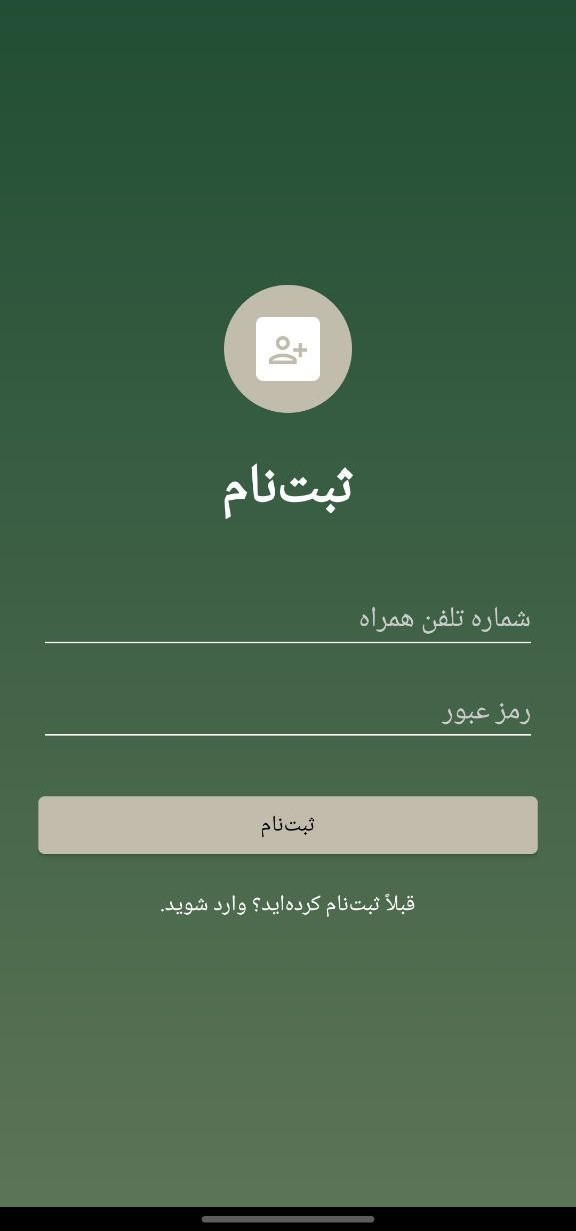
\includegraphics[width=0.7\textwidth,height=10cm,keepaspectratio]{Pic/signup}
		\caption{ثبت نام}
		\label{fig:signup}
	\end{subfigure}
	\begin{subfigure}[b]{0.3\textwidth}\centering
		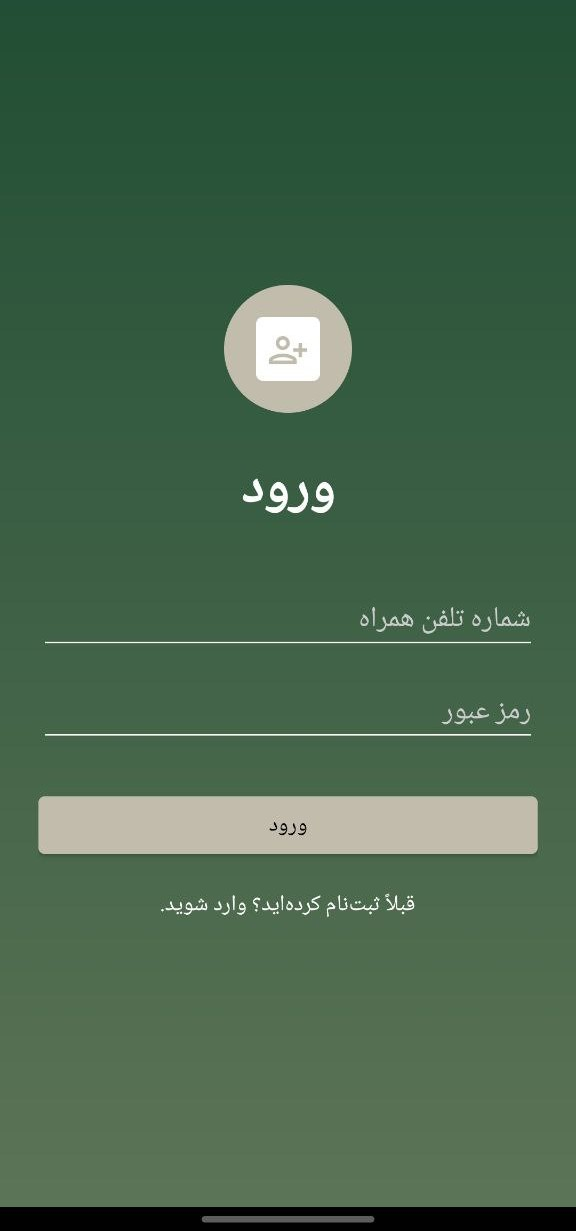
\includegraphics[width=0.7\textwidth,height=10cm,keepaspectratio]{Pic/login}
		\caption{ورود}
		\label{fig:login}
	\end{subfigure}
	\caption{اولین صفحات مشاهده شده}
	\label{fig:animals}
\end{figure}

\begin{itemize}
	\item \textbf{ثبت‌نام:}\\
	کاربر باید شماره تلفن همراه و رمز عبور خود را وارد کرده و اقدام به ایجاد حساب کاربری جدید نماید. رمز عبور باید حداقل شش کاراکتر داشته. درصورت داشتن اکانت، با لمس عبارت \textbf{«قبلاً ثبت‌نام کرده‌اید؟ وارد شوید.»} وارد صفحه ورود  شده.
	
	\item \textbf{ورود:}\\
	همانند صفحه ثبت نام با وارد کردن شماره تلفن همراه و رمزعبور وارد امانت خود شده. درصورت نداشتن اکانت، با لمس عبارت \textbf{«حساب ندارید؟ ثبت‌نام کنید.»} وارد صفحه ورود  شده.
\end{itemize}

\section{محیط اصلی}

\subsection{تنظیمات}

برنامه تنظیمات به شما امکان می‌دهد رنگ‌ها و مقادیر سطح مربوط به آن‌ها را برای نمایش داده‌های شبکه تنظیم کنید. 
این تنظیمات در سه مرحله اصلی انجام می‌شود: انتخاب گزینه‌ها، انتخاب رنگ‌ها، و ثبت نهایی. 

\begin{itemize}
	\item \textbf{انتخاب گزینه‌ها} \\
	در بالای صفحه، سه بخش برای انتخاب گزینه‌های اصلی وجود دارد:
	
	\begin{itemize}
		\item \textbf{تکنولوژی:} از منوی کشویی اول، نسل شبکه مورد نظر را انتخاب کنید. گزینه‌های موجود 2G، 3G، 4G و 5G هستند.
		\item \textbf{ویژگی:} با توجه به انتخاب شما در مرحله قبل، منوی کشویی دوم به‌روز می‌شود. این منو شامل انواع سیگنال‌های مربوط به تکنولوژی انتخابی است. به عنوان مثال، برای 4G، می‌توانید rsrp یا rsrq را انتخاب کنید.
		\item \textbf{تعداد رنگ‌ها:} از منوی کشویی سوم، تعداد سطوح مختلف کیفیت سیگنال را که می‌خواهید تعریف کنید، انتخاب کنید. این عدد بین 3 تا 50 قابل تغییر است و تعداد رنگ‌هایی را که باید به سیستم اضافه کنید، مشخص می‌کند.
	\end{itemize}
	\item \textbf{انتخاب و تعریف رنگ‌ها:}
	\begin{itemize}
		\item \textbf{انتخاب رنگ:} از چرخ رنگی بزرگ میانی استفاده کنید تا رنگ مورد نظر خود را برای یک سطح خاص از کیفیت سیگنال انتخاب کنید.
		\item \textbf{تعریف مقادیر:} پس از انتخاب رنگ، دکمه \textbf{افزودن رنگ} را فشار دهید. یک کادر گفت‌وگو ظاهر می‌شود که از شما می‌خواهد سه مقدار را وارد کنید:
		\begin{itemize}
			\item \textbf{عدد سطح:} عددی برای رتبه‌بندی کیفیت (مثلاً ۱ برای ضعیف، ۲ برای متوسط و ۳ برای خوب). هر رنگ باید یک عدد سطح یکتا داشته باشد.
			\item \textbf{حداقل مقدار بازه:} پایین‌ترین مقدار عددی برای این سطح کیفیت.
			\item \textbf{حداکثر مقدار بازه:} بالاترین مقدار عددی برای این سطح کیفیت.
		\end{itemize}
	\end{itemize}

	\item \textbf{ویرایش و نهایی کردن:}
	\begin{itemize}
		\item پس از افزودن هر رنگ، یک جعبه کوچک با رنگ انتخابی و عدد سطح آن در پایین چرخ رنگی نمایش داده می‌شود.
		\item برای ویرایش یک رنگ تعریف شده، روی جعبه رنگ مربوطه کلیک کنید. با این کار، رنگ در چرخ رنگی انتخاب می‌شود و می‌توانید با فشار مجدد دکمه \textbf{افزودن رنگ}، مقادیر آن را تغییر دهید. درصورت منصرف شدن از ویرایش با کلیک دوباره بر رنگ از حالت ویرایش خارج میشوید.
		\item زمانی که تعداد رنگ‌های انتخابی شما با عددی که در مرحله اول انتخاب کرده‌اید برابر شود، یک دکمه \textbf{ثبت نهایی} ظاهر می‌شود.
	\end{itemize}
	
	
\end{itemize}

\begin{figure}[ht]
	\centering
	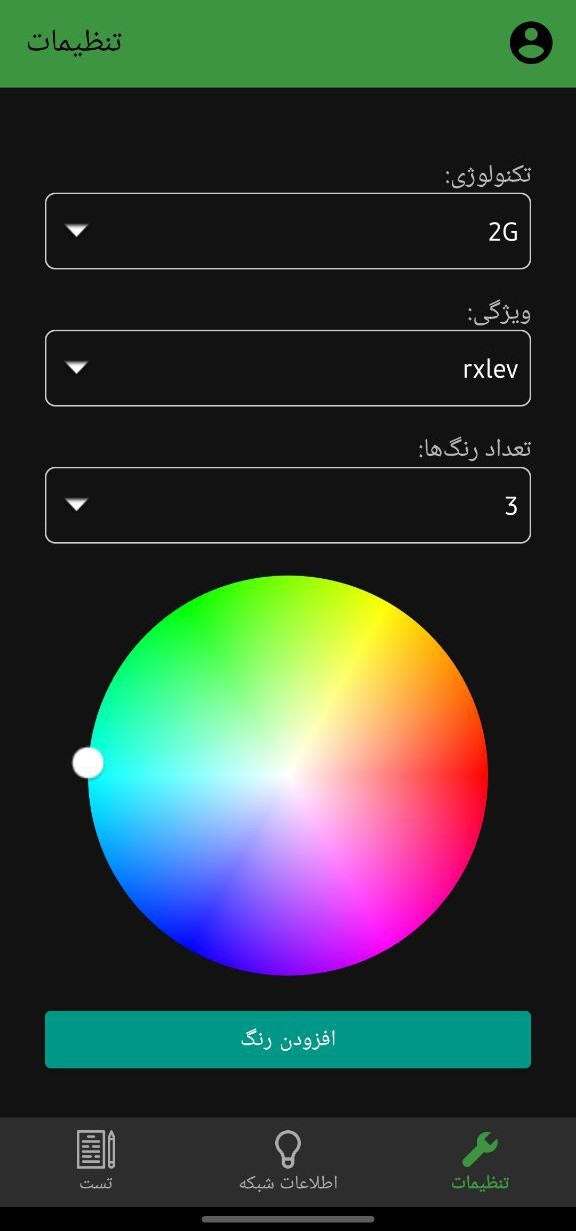
\includegraphics[width=0.7\textwidth,height=10cm,keepaspectratio]{Pic/setting}
	\caption{صفحه تنظیمات شبکه}
	\label{fig:setting}
\end{figure}

\subsection{اطلاعات شبکه}

در صفحه اطلاعات، وضعیت شبکه و موقعیت جغرافیایی کاربر به صورت زنده نمایش داده می‌شود.  
با فشردن دکمه \textbf{نمایش در نقشه}، موقعیت فعلی کاربر روی نقشه نشان داده می‌شود.

این اطلاعات به طور خودکار در پس‌زمینه به سرور ارسال می‌شوند و در همین صفحه می‌توان داده‌های ارسالی را مشاهده کرد.

\begin{figure}[ht]
	\centering
		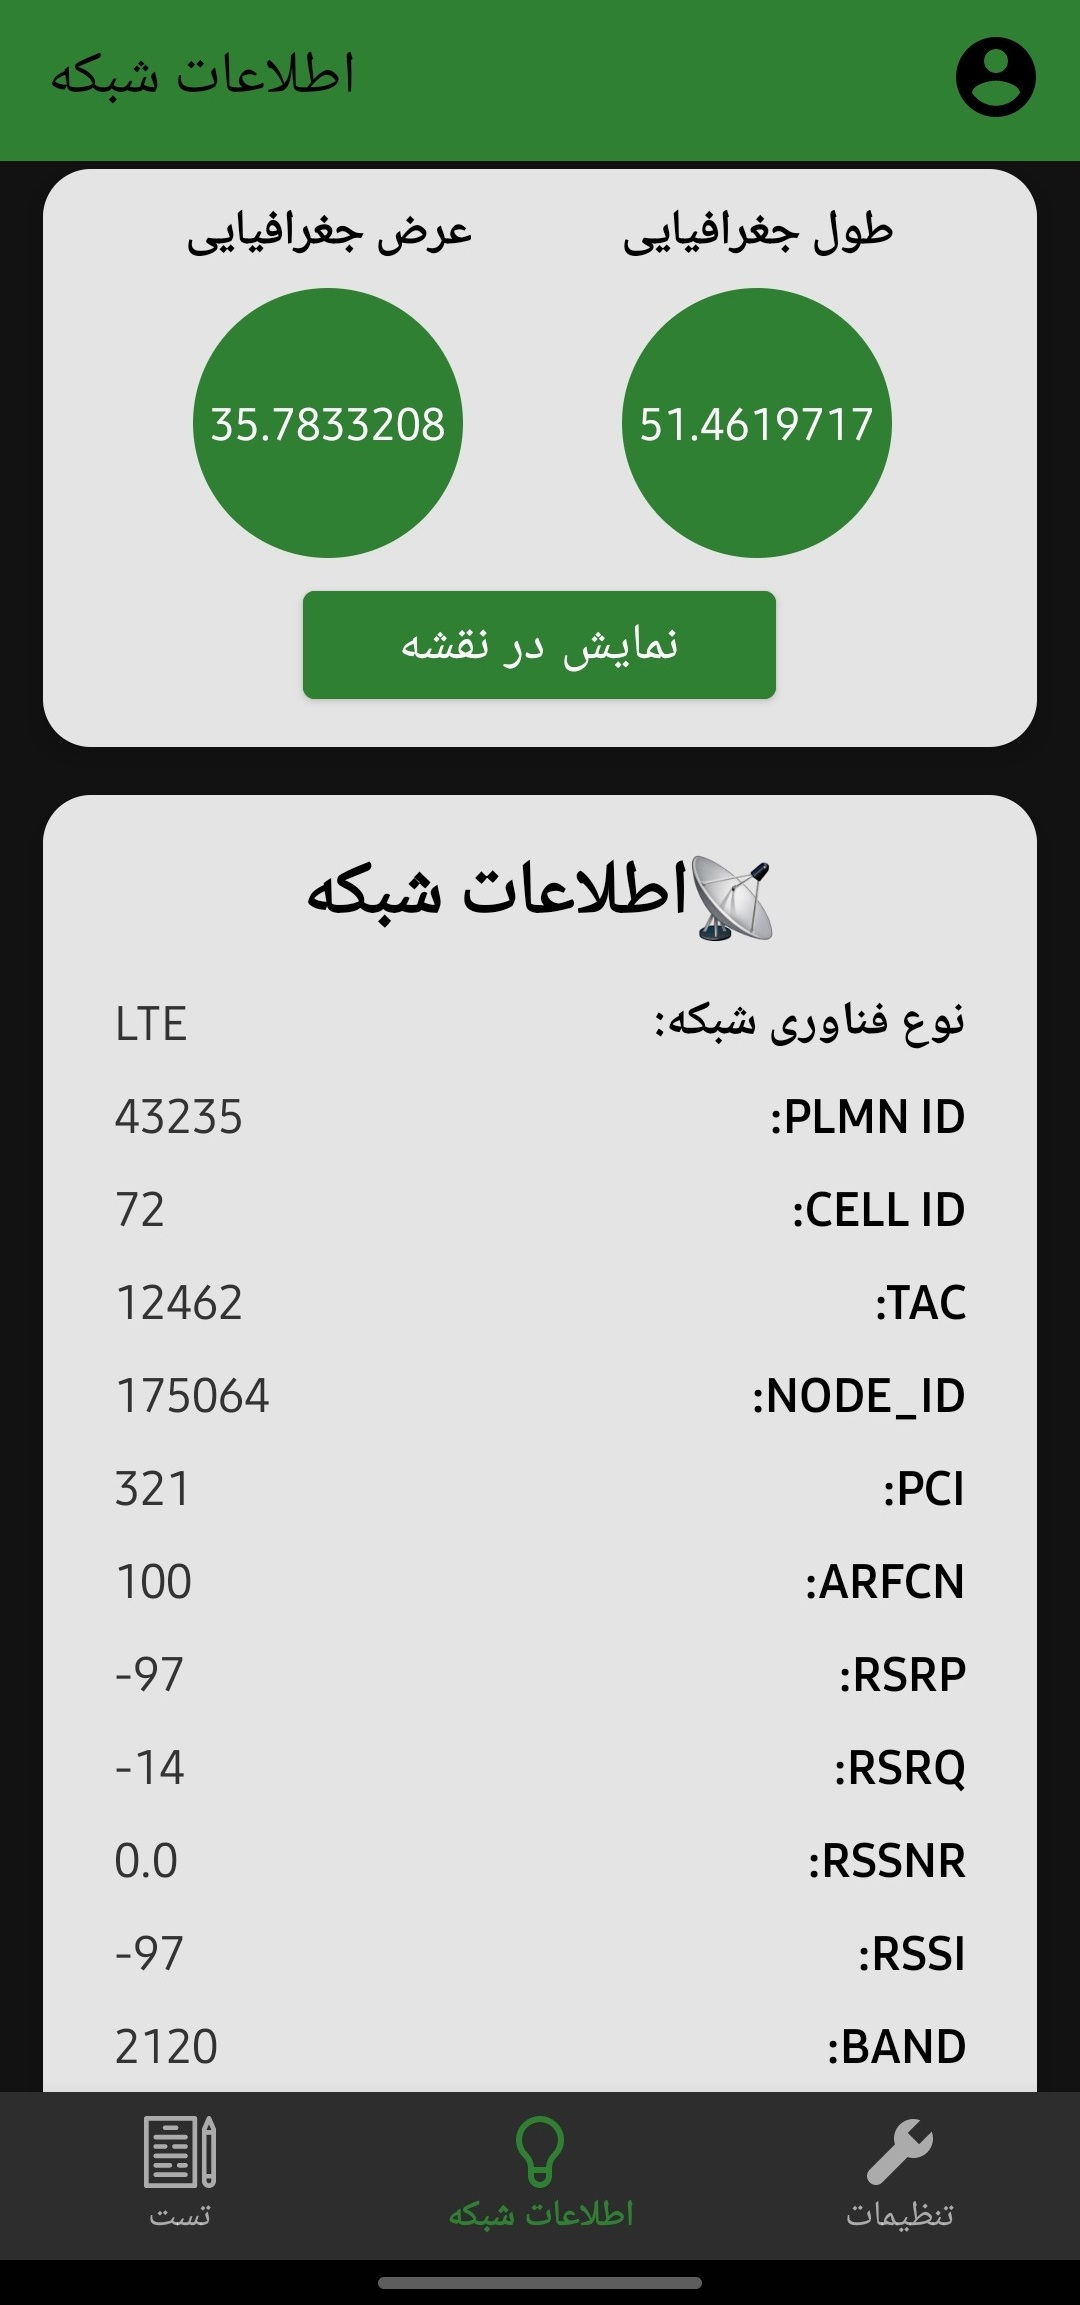
\includegraphics[width=0.7\textwidth,height=10cm,keepaspectratio]{Pic/info}
	\caption{صفحه اطلاعات شبکه}
	\label{fig:info}
\end{figure}

\subsection{تست‌ها}

با استفاده از این برنامه می‌توانید عملکرد و وضعیت شبکه اینترنت خود را با انجام تست‌های مختلف، به صورت دقیق بررسی کنید.

\begin{itemize}
	\item \textbf{بخش «تست‌های شبکه»} 

این بخش شامل شش دکمه برای انجام تست‌های مختلف شبکه است که می‌توانید به راحتی هر کدام را انتخاب و اجرا کنید.

\begin{itemize}
	\item \textbf{گذردهی دانلود (\lr{Download Throughput}):}\\
	با کلیک روی این دکمه، سرعت \textbf{دانلود داده} از سرور به گوشی شما سنجیده می‌شود. این تست برای ارزیابی عملکرد شبکه در هنگام دریافت فایل‌ها یا پخش ویدیو مفید است.
	
	\item \textbf{گذردهی آپلود (\lr{Upload Throughput}):}\\
	با کلیک روی این دکمه، سرعت \textbf{آپلود داده} از گوشی شما به سرور اندازه‌گیری می‌شود. این تست برای بررسی عملکرد شبکه در هنگام ارسال فایل‌ها یا آپلود تصاویر در شبکه‌های اجتماعی کاربرد دارد.
	
	\item \textbf{:Ping}\\
	این دکمه برای بررسی \textbf{زمان تأخیر (Latency)} در اتصال شبکه شما به یک سرور خاص به کار می‌رود. هرچه مقدار پینگ کمتر باشد، زمان پاسخ‌دهی شبکه بهتر است.
	
	\item \textbf{:DNS}\\
	این تست سرعت \textbf{پاسخ‌دهی سرور DNS} را می‌سنجد. DNS آدرس‌های وب ( \lr{www.google.com}) را به آدرس‌های IP ترجمه می‌کند. سرعت بالای پاسخ‌دهی DNS باعث لود شدن سریع‌تر صفحات وب می‌شود.
	
	\item \textbf{:Web}\\
	با کلیک روی این دکمه، عملکرد و سرعت \textbf{بارگذاری یک صفحه وب} مشخص تست می‌شود. این تست برای شبیه‌سازی تجربه واقعی کاربر هنگام مرور اینترنت طراحی شده است.
	
	\item \textbf{:SMS}\\
	این تست \textbf{سرعت ارسال پیامک (SMS)} را بررسی می‌کند. با این تست می‌توانید اطمینان حاصل کنید که سرویس پیامکی شما به درستی کار می‌کند.
	 \begin{figure}[ht]
		\centering
		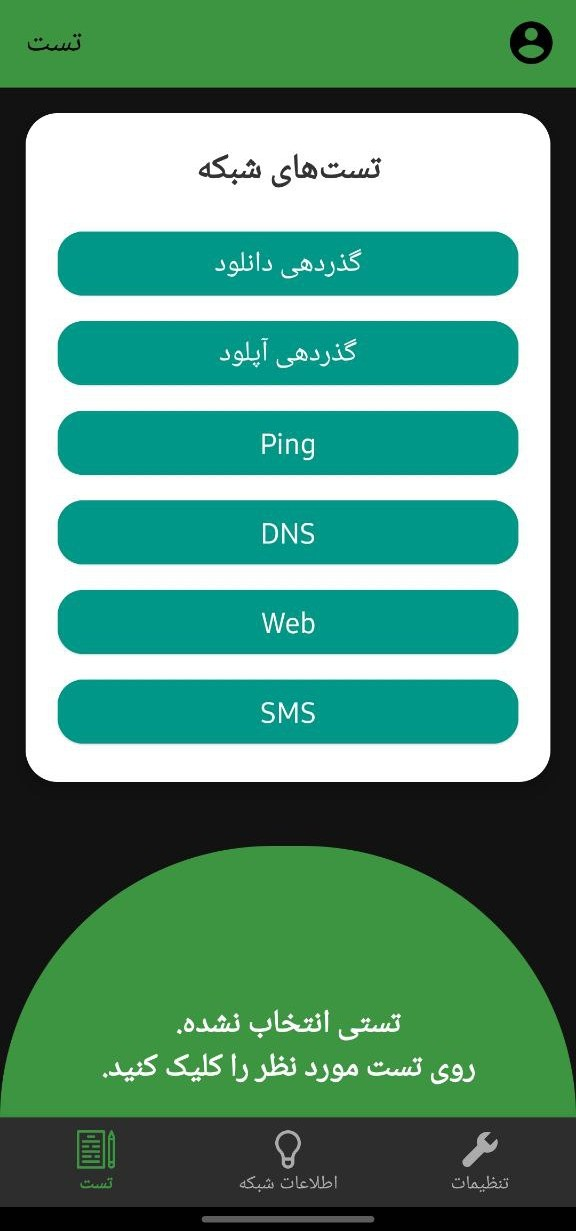
\includegraphics[width=0.7\textwidth,height=10cm,keepaspectratio]{Pic/test}
		\caption{صفحه تست ها}
		\label{fig:test}
	\end{figure}
\end{itemize}

\item \textbf{بخش «نتیجه تست»}  
در این بخش، نتایج تست‌های اجراشده نمایش داده می‌شود.\\
پیش از شروع هر تست، پیامی ظاهر می‌شود که از شما می‌خواهد روی دکمه موردنظر کلیک کنید.\\
هر تست در بازه‌ای دو دقیقه‌ای اجرا می‌شود و بین مراحل آن تأخیری ۱۰ ثانیه‌ای وجود دارد. 
به همین دلیل، پس از شروع یک تست، سایر دکمه‌ها تا پایان زمان دو دقیقه غیرفعال خواهند بود.\\

همچنین توجه داشته باشید که اگر هنگام اجرای تست از صفحه خارج شوید، فرآیند تست ناتمام باقی خواهد ماند.
\end{itemize}

\subsection{مدیریت حساب کاربری}

این صفحه به شما امکان می‌دهد اطلاعات حساب کاربری خود را مشاهده و مدیریت کنید.

\begin{itemize}
	\item \textbf{مشاهده و ویرایش اطلاعات حساب:}  
	در بخش میانی صفحه، سه فیلد برای نمایش اطلاعات شما وجود دارد:
	\begin{itemize}
		\item \textbf{شماره تلفن همراه:} شماره تلفن همراه کنونی، که با آن ثبت نام کرده اید را نشان می دهد.
		\item \textbf{رمز عبور:} رمز عبور شما به صورت محرمانه و با ستاره نمایش داده می‌شود.
		\item \textbf{نقش:} یکی از دو نقش "کاربر" یا " ادمین نشان که نشان دهنده دسترسی های شما هست.
	\end{itemize}
	
	\item \textbf{خروج از حساب:}  
	در پایین صفحه، یک دکمه با عنوان \textbf{«خروج»} وجود دارد. با ضربه زدن روی این دکمه، شما از حساب کاربری خود خارج خواهید شد.
\end{itemize}

 
  \begin{figure}[ht]
 	\centering
 	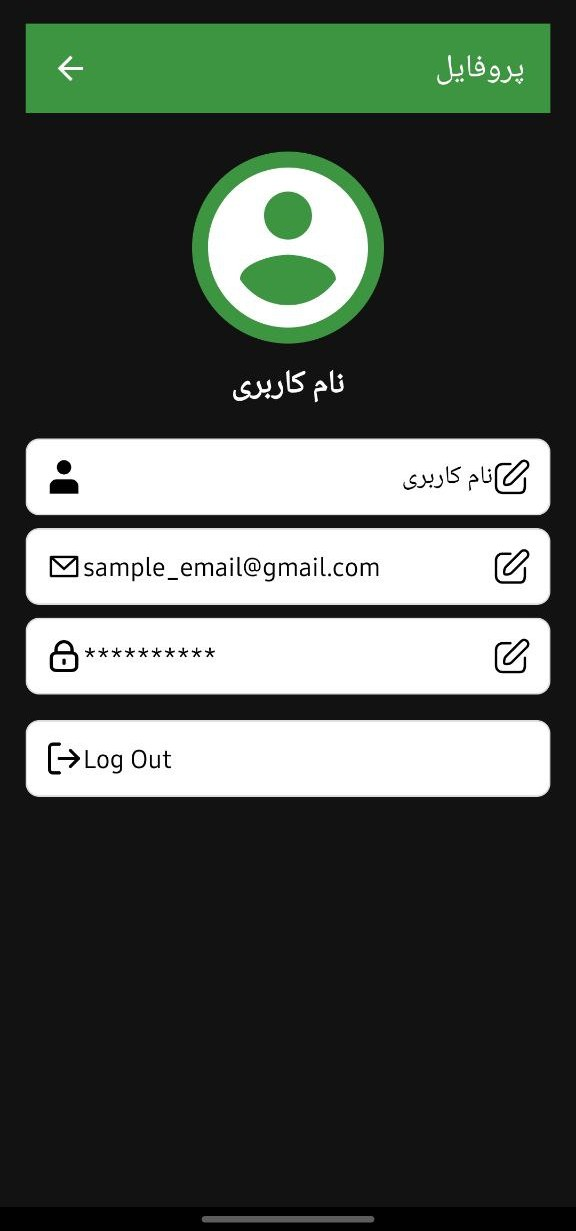
\includegraphics[width=0.7\textwidth,height=10cm,keepaspectratio]{Pic/profile}
 	\caption{صفحه حساب کاربری}
 	\label{fig:profile}
 \end{figure}
\end{document}



